%************************************************
\chapter{Introduction}\label{ch:introduction}
%************************************************
\section{Motivation}
In recent years, there has been a rise in the use of neuroimaging in the clinical practice. It has improved and speeded the procedure of diagnostic, providing unprecedented insight into the brain. Neuroimaging is a very extended tool in research as well. Different fields such as psychiatry, neurology, psychology, behavioural science or biology make extensive use of brain imaging in their studies. 

The basis of these studies are common: a selection procedure by which a representative set of subjects is recruited, a performance of the experiment on (or by) each subject and a statistical analysis of the acquired data. Particularly, when studying a certain disease, it is common to recruit subjects affected by the disease and non-affected, healthy subjects, usually known as \acp{CTL}. Then, in this typical example, both affected and \acp{CTL} are scanned, and brain anatomy or function is analysed using statistical tools. The result of this analysis is a list of significant differences between structure or function that are linked to the disease. 

\ac{CAD} systems provide a set of tools to help setting up and performing these studies. It is currently a thriving area of research involving multidisciplinary teams, combining computer science, mathematics, medicine, artificial intelligence, statistics, machine learning, and many others. The main aim is to assist clinicians in the procedure of diagnosis and study of the diseases by providing software that can effectively recognize disease patterns, characterize differences and make predictions. 
\cite{Martinez-Murcia2016}

One fundamental issue often found in this studies is the sample size. The number of subjects frequently ranges from tens to hundreds, whereas the number of features (namely voxels) to be analysed can add up to millions. This causes the so-called \emph{Small Sample Size Problem} \cite{Duin2000} which negatively affects the statistical power of any experiment performed using these datasets \cite{Button2013}. 

\subsection{The Small Sample Size Problem}
The Small Sample Size Problem arises as a loss of statistical power when the number of samples is small compared to the number of features. This loss of statistical power translates to neuroimaging as false positives (the system detects signal where there is not) or false negatives (the system is unable to detect some signals). In differential diagnosis studies, it leads to places where differences are stated where there is not 

In addition to some confounding effects, such as population bias or scanner differences, 


Solucion tipica: multilple comparison correction. 



Main idea: Neuroimaging studies need are subject to the small sample size problem. To overcome that problem we must either decrease the number of features or increase the sample size. 


FromChapter: Signal decomposition techniques are widely used in many applications, ranging from one-dimensional signals such as audio or electroencephalography (EEG) to multidimensional arrays, and are frequently applied as feature reduction to overcome the small sample-size problem, that is, the loss of statistical power due to a larger number of features compared to the number of samples.


\section{Neuroimaging Modalities}
There exist a variety of imaging modalities used in neuroscience. By far, the most extended is \ac{MRI}, which provides intensity maps that represent the internal structure of the brain. Other modalities are aimed at studying the function of the brain, by injecting radioactive ligands that, linked to a receptor, can measure its distribution. This is the case of \ac{PET} and \ac{SPECT}.

\subsection{Magnetic Resonance Imaging}
\acf{MRI} is perhaps the most widespread imaging modality, and it is used to analyse both structural and functional properties of the brain. 

\begin{figure}[htp]
\centering
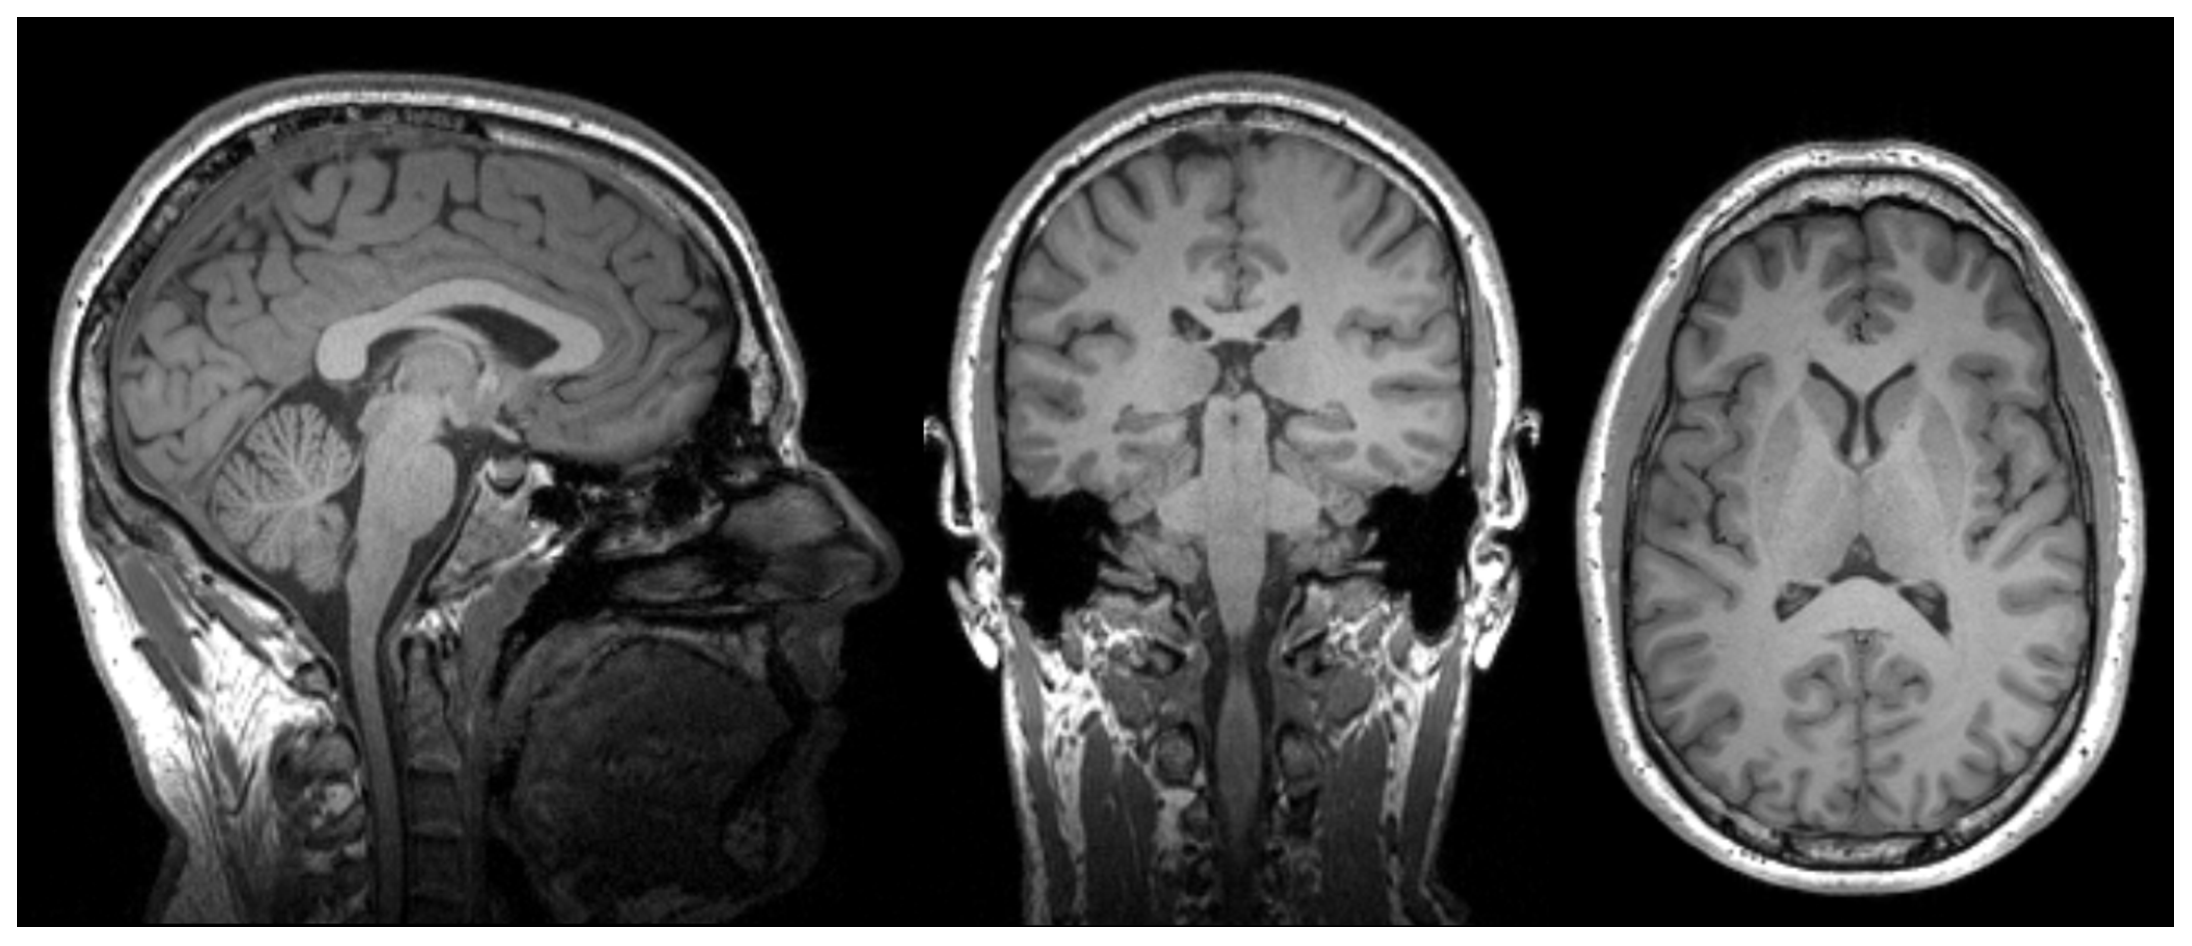
\includegraphics[width=0.7\linewidth]{gfx/ch1/example_MRIT1}
\caption[Example of a T1-weighted MRI image.]{Example of a T1-weighted MRI image.}
\label{fig:example_MRI}
\end{figure}


Technology. Physics fundamentals. 

\subsection{Single Photon Emission Computed Tomography}
\acf{SPECT} is 

Ref: has been the cornerstone of nuclear medicine and it is widely used to detect molecular changes in cardiovascular, oncological and neurological diseases.

Technology. 

Radiotracers used. Here: DATSCAN. HMPAO. 

\subsection{Positron Emission Tomography}
\subsection{Other Modalities}

\section{Machine Learning in Neuroimaging}
In contrast to traditional visual inspection a semiquantitative analysis of neuroimaging, machine learning is nowadays a trend in the field. Machine learning is the subfield of computer science that provides computers with the ability to learn from data instead of being programmed for an explicit task. Applications range from automatic processing of images to \acf{CAD}, 

Statistical techniques such as \ac{PCA}, are used for feature extraction and hypothesis testing for feature selection in systems intended to 

\ac{CAD}

\section{Overview}
This thesis explores how to use signal processing and machine learning to overcome the small sample size problem in neuroimaging. 

First strategy: decrease the number of features -> Feature extraction. This is the subject of Decomposition techniques, Texture Analysis and \ac{SBM}. 

Second strategy: increase the sample size. Most popular option: multi-site studies where subjects are acquired using similar techniques at different sites. This poses a major problem: inhomogeneities, etc. To overcome this we propose the \ac{SWPCA}. Other option: simulate new subjects from the existent database, in order to increase sample size. 